\setcounter{footnote}{0}
\setcounter{figure}{0}
\setcounter{table}{0}
\chapter*{Uma análise de metacontingências e macrocontingências envolvidas em práticas de gênero}
\addcontentsline{toc}{chapter}{Capítulo 7}
\addcontentsline{toc}{section}{Uma análise de metacontingências e macrocontingências envolvidas em práticas de gênero}
\addcontentsline{toc}{subsection}{\textbf{Autoras:} \textit{Júlia Cavalcanti Ferraz, Hellen Luane Silva \\Peixinho, Christian Vichi \& Angelo A. S. Sampaio }}
\begin{flushright}
\begin{small}
    Júlia Cavalcanti Ferraz\\
    Hellen Luane Silva Peixinho\\
    Christian Vichi\\
    Angelo A. S. Sampaio\\
\end{small}
\vspace{1cm}
\end{flushright}

A visão de comportamento humano na perspectiva behaviorista radical envolve a consideração de sua multideterminação em três níveis distintos, mas inter-relacionados: (1) filogênese, que se refere às características selecionadas na história da espécie; (2) ontogênese, que envolve processos comportamentais que produzem repertórios novos e adaptativos ao ambiente do indivíduo; e (3) cultura, que diz respeito ao ambiente social que, principalmente por meio da linguagem, possibilita a aquisição de novos comportamentos, sem a necessidade de exposição prévia às contingências operantes (Skinner, 1981; Tourinho, 2003), bem como a seleção de operantes entrelaçados de diferentes indivíduos enquanto unidade cultural (Glenn et al., 2016).

A importância da cultura para a compreensão do comportamento humano é destacada por Skinner (e.g., 1953/2007, 1971, 1981) em diversos momentos de sua obra, inclusive apontando restrições sociais do papel de dona de casa, em seu livro Walden II (Skinner, 1948). Mais recentemente, Daly (1996) discutiu práticas sexistas, abordagens teóricas do feminismo e práticas culturais. Os analistas do comportamento também têm destacado a importância de intervenções sobre questões sociais, apesar de pouco esforço ter sido feito no sentido de intervir sobre as práticas de gênero (Ruiz, 1998; Wolpert, 2005). Uma exceção notável foi o trabalho de Maria Ruiz, que discutiu e relacionou feminismo e behaviorismo radical em periódicos científicos da área (Ruiz, 1995, 1998, 2003, 2009; Ruiz \& Roche, 2007).

Visando remediar a lacuna de estudos sobre práticas de gênero, esse trabalho analisa o tema à luz da Análise Comportamental da Cultura. Para esse fim, é importante definir e operacionalizar brevemente alguns conceitos, visando descrever detalhadamente os fenômenos de interesse – sem pretensão, contudo, de findar as discussões acerca dos temas envolvidos.

\section*{Sexo, Gênero, Prática de Gênero, Feminismo e Planejamento Cultural}

O sexo de um indivíduo é determinado por três critérios distintos: genético, morfológico e funcional. O critério genético refere-se aos cromossomos sexuais que um indivíduo carrega, geralmente, XX para mulheres e XY para homens. O critério morfológico está relacionado à anatomia dos órgãos genitais e à presença de características sexuais secundárias, desenvolvidas durante a puberdade, como tamanho e aparência dos pelos, desenvolvimento das mamas e timbre da voz (Snustad \& Simmons, 2012), podendo ou não implicar em correspondência com o critério genético. Ou seja, existem indivíduos com carga genética XY que apresentam morfologia tipicamente feminina e indivíduos XX que apresentam morfologia masculina (Snustad \& Simmons, 2012) – o que indica que, mesmo biologicamente, não é tão simples determinar o sexo de um indivíduo. O critério funcional é definido quando, diante da presença de genitália masculina e/ou feminina, avalia-se se esse(s) órgão(s) está(ão) em seu devido funcionamento biológico. Geralmente, os critérios morfológico e funcional afetam a probabilidade de um indivíduo ser considerado socialmente como homem ou mulher.

Seguindo tal raciocínio o sexo pode ser considerado uma construção social, o que, segundo Ruiz (2003), também se aplica à noção de gênero. Este emerge de um conjunto de práticas culturais e, principalmente, verbais. O conceito de gênero, por sua vez, refere-se a padrões comportamentais “modelados e mantidos por contingências sociais e padrões de reforçamento dentro da comunidade verbal” (Ruiz, 2003, p. 12) de acordo com o sexo de um indivíduo. Essa definição de gênero é importante, pois dialoga com concepções antiessencialistas também presentes nas obras de feministas (Laurenti \& Silva, 2016). Um exemplo dentro do feminismo foi a obra de Simone de Beauvoir (1949/1970), que advogou não haver um modelo único e ideal que seja capaz de definir o que é a mulher, ou seja, não existe uma essência feminina que determine os padrões de comportamento típicos para uma mulher. Skinner (1981), por sua vez, criticou explicações da subjetividade dos indivíduos partindo de uma essência interna (em uma visão mentalista) e propôs seu modelo de seleção pelas consequências, em que os padrões comportamentais de uma pessoa são selecionados e mantidos pelas consequências que os produzem (Laurenti \& Silva, 2016).

Práticas de gênero podem ser caracterizadas como comportamentos sob um controle condicional específico: observadores tendem a interpretar e reagir diferentemente a um mesmo comportamento, a depender do sexo do emitente. Ou seja, o sexo de um indivíduo seria um estímulo condicional que evoca diferentes comportamentos no mesmo observador (Ruiz, 1998, 2003).

Um exemplo de prática de gênero pode ser inferido a partir de dados estatísticos brasileiros sobre o pagamento de salários desiguais para homens e mulheres que ocupam a mesma profissão. A Pesquisa Nacional por Amostra de Domicílios (Instituto Brasileiro de Geografia e Estatística, 2016) constatou que “o rendimento médio mensal real de todos os trabalhos dos homens de 15 anos ou mais de idade, com rendimento de trabalho, foi de R\$2.058 e o das mulheres, R\$1.567” (p. 69) e que, em média, as mulheres receberam o equivalente a 76,1\% do rendimento de trabalho dos homens em 2015. Em contraste com essa diferença salarial, o número médio de anos de estudo das mulheres foi maior que o observado entre os homens (8,0 e 7,6 anos, respectivamente). Ou seja, apesar de passarem, em média, mais tempo se dedicando aos estudos, ao chegar no mercado de trabalho as mulheres recebem salários significativamente inferiores aos dos homens. Outro exemplo de diferença salarial pode ser encontrada em um estudo feito com profissionais da enfermagem, profissão tipicamente considerada “feminina”, com dados dos anos de 1988 a 2013, nos Estados Unidos, onde 7\% da amostra era de homens e os salários masculinos eram maiores que os salários femininos durante todos os anos, chegando a uma diferença média de 11,26\%, sem mudanças estatisticamente significativas nessa lacuna salarial ao longo do tempo (Muench et al., 2015). Apesar desses dados, sozinhos, não controlarem variáveis como cargo, experiência profissional e o tamanho ou prestígio das empresas nas quais mulheres e homens trabalham, eles sugerem que a definição da remuneração paga é afetada pelo sexo do trabalhador.

Práticas de gênero podem ser explicitamente coercitivas, quando consequências aversivas são apresentadas para pessoas de determinado sexo que não se comportem de acordo com o padrão esperado para o respectivo gênero. Sidman (1989/2009) descreveu o controle verbal coercitivo envolvido na modelagem de repertórios de gênero feminino e masculino. Ele destacou, por exemplo, a forma com que muitos psiquiatras rotularam a recusa de mulheres em desempenhar um papel tradicional nas relações entre os sexos (e.g., ser passiva, desejar ser esposa, mãe, dona-de-casa, etc.) como não-saudável, sendo, portanto, objeto de intervenção. Além disso, Sidman descreveu o uso do controle coercitivo contra mulheres que não se comportam da maneira que é esperada, destacando que “os padrões absolutos de normalidade feminina são baseados em tradição cultural, não em análise científica” (p. 195).

As práticas de gênero muitas vezes envolvem um controle condicional discreto (Ruiz, 2003). Isso decorre das práticas de gênero geralmente envolverem um controle condicional no qual o sexo estabelece uma relação estímulo-estímulo. Ou seja, um indivíduo aprende a responder a determinados comportamentos de terceiros, por exemplo, a punir o comportamento de uma pessoa ao sentar de pernas abertas, mas a resposta varia em função do sexo de quem se comporta, homens sentados de pernas abertas não costumam sofrer punição, diferente de mulheres se comportando da mesma forma. O mesmo acontece em relação a outras características físicas ou étnicas que dão base para determinadas práticas culturais discriminatórias. Ruiz (2003) argumenta que essas relações condicionais discretas evocadas pelo sexo, encontradas no controle condicional de práticas de gênero, dificulta que o indivíduo seja capaz de tatear as contingências que controlam o seu comportamento. 

Outra definição relevante é a de feminismo, aqui entendido como um conjunto de práticas culturais que têm como objetivo alterar o papel social da mulher, com base em ações que tornem explícitas as práticas culturais de gênero, responsáveis por um desequilíbrio na distribuição e alocação de reforçadores, de forma favorável aos homens (Fideles \& Vandenberghe, 2014; Ruiz, 2003; Silva \& Laurenti, 2016). Nesse sentido, o feminismo pode ser entendido como uma forma de contracontrole social em relação às práticas de gênero. Contracontrole social é definido como uma classe de respostas emitida por um indivíduo ou grupo de indivíduos que tenha como efeito a prevenção, eliminação ou atenuação das consequências aversivas às quais estão submetidos, principalmente aquelas consequências de exploração produzidas por um determinado meio de controle social institucionalizado (legal ou habitual) ou em vias de institucionalização (Sá, 2016). O feminismo seria uma forma de contracontrole social que busca explicitar e modificar as fontes de controle e as consequências acumuladas a longo prazo que reduzem os reforçadores para as mulheres.

Wolpert (2005) destaca os riscos de ignorar fontes de controle relacionadas ao gênero, raça e classe social ao analisar práticas sociais e executar planejamentos culturais em uma sociedade, tendo em vista o papel fundamental dessas fontes de controle nas contingências cotidianas de reforçamento. A análise de Ruiz (2003) se mostra importante para elucidar tais fontes discretas de controle no que diz respeito ao gênero, já que desconsiderá-las em uma análise cultural tornaria o planejamento cultural incompleto e menos eficaz (Wolpert, 2005). As duas autoras apontam o Behaviorismo Radical como uma base filosófica adequada para a compreensão destas práticas, visto que se trata de uma filosofia da ciência contextualista, entendendo o ser humano dentro de sua história de vida e contingências atuais (Ruiz, 2003; Wolpert, 2005).

A análise do terceiro nível de seleção já vem sendo realizada em uma perspectiva behaviorista (Baum, 2006; Glenn, 1986, 2004; Pierce, 1991; Todorov, 2012) e os conceitos propostos por Glenn et al. (2016) podem nortear uma análise de práticas culturais de gênero. De acordo com Glenn et al., os conceitos de metacontingência e macrocontingência, apesar de não serem os únicos possíveis para a compreensão das práticas culturais, “têm sido ferramentas conceituais úteis tanto em guiar análises experimentais, quanto na compreensão e mudança cotidiana dos problemas no nível cultural” (p. 12).

\section*{Metacontingências e Macrocontingências relacionadas às Práticas de Gênero}

O conceito de metacontingência diz respeito às relações contingentes entre (1) contingências comportamentais entrelaçadas (CCEs) recorrentes, gerando certo produto agregado (PA), e (2) eventos ou condições ambientais selecionadoras (Glenn et al., 2016). As CCEs envolvem comportamentos de duas pessoas ou mais, em que a resposta de uma, ou seus efeitos, servem de ambiente para o comportamento de uma outra, e assim por diante, tendo como resultado desta interação um PA que não seria possível sem este entrelaçamento (Glenn et al., 2016). 

Já uma macrocontingência envolve a “relação entre (1) comportamentos operantes controlados por contingências individuais e/ou CCEs governadas por metacontingências e (2) um efeito cumulativo de significância social” (Glenn et al., 2016, p. 19). O primeiro termo de uma macrocontingência pode ser denominado de macrocomportamento\linebreak (Glenn et al., 2016). 

Como as práticas de gênero são bastante diversas e complexas, propomos uma interpretação de apenas duas delas: uma, chamada de “assédio sexual verbal”, foi escolhida devido a ter sido tratada na legislação brasileira recente; a outra, conhecida por “currículo oculto”, teve uma análise inicial feita por Ruiz (2003), mas exige uma análise mais aprofundada. Embora Ruiz (1998, 2003) fale em termos de metacontingências ao se referir ao currículo oculto, pois se trata de um produto de ações entrelaçadas, esta prática parece se enquadrar melhor no conceito de macrocontingência. Esta pode englobar metacontingências que, por sua vez, podem estar associadas a contingências operantes individuais recorrentes, contribuindo para o efeito cumulativo da restrição do acesso das mulheres a fontes de reforçadores e alocação de recursos ao qual Ruiz (2003) se refere.

Quando linhagens operantes de um certo número de pessoas são similares o suficiente em forma ou produto, isso pode ser chamado de uma prática cultural. Isso pode se tornar um problema social se o comportamento constituinte da prática tem um efeito cumulativo que pode afetar outras pessoas, sendo perigoso ou prejudicial para a saúde, segurança ou felicidade de um grande número de pessoas (Glenn et al., 2016; Malott \& Glenn, 2006). Por exemplo, o uso de controle aversivo, como punições constantes do comportamento de mulheres, pode levar ao efeito cumulativo de agravo na saúde mental dessa população. Isso não implica, contudo, que esse efeito cumulativo funcione como consequência que mantém o macrocomportamento constituinte da prática ou linhagem culturo-comportamental, ou seja, não há uma relação propriamente de contingência entre o macrocomportamento e seu efeito cumulativo.

\section*{O Currículo Oculto nas Escolas}

Os estudos de Sadker e Sadker (1994) avaliaram as relações entre professor-aluno em várias escolas nos Estados Unidos e demonstraram diferentes distribuições de privilégios manejados por professores de acordo com o sexo da criança. Especificamente as crianças do sexo masculino eram favorecidas em sala de aula, pois recebiam claramente uma proporção consideravelmente maior de recursos manejados pelos professores (e.g., atenção, feedback positivo, correção de respostas, reforçadores sociais, etc.) em relação ao seu desempenho acadêmico, enquanto que, para as crianças do sexo feminino, os mesmos reforçadores são relacionados mais a questões como “bom comportamento”, estética e caligrafia.

Neste cenário, os professores relataram não perceber que o sexo da criança exercia controle condicional em sua prática profissional. Ou seja, os professores não eram capazes de tatear as contingências que administravam diferencialmente com frequência. O fato desse controle não ser detectado (tateado) por parte dos sujeitos, nos dá uma noção da sutileza do controle exercido pelas práticas de gênero sobre o comportamento. Este é um dos exemplos de práticas educacionais que compõem a macrocontingência do que foi denominado de currículo oculto (Figura \ref{figura1}; Ruiz, 2003).

\begin{figure}[ht]
    \begin{center}
        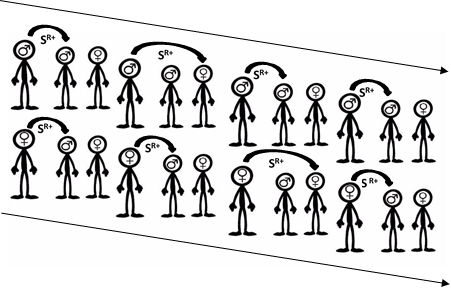
\includegraphics[width=0.7\textwidth]{7/figura1}
        \captionof{figure}{Esquema da prática conhecida como currículo oculto, baseado nos estudos de Sadker e Sadker (1994) e na análise de Ruiz (2003). As setas provenientes das pessoas maiores (professores) em direção ao menino ou à menina representam recursos (reforçadores no geral) manejados por professores. As setas diagonais indicam a transmissão da prática ao longo de gerações de professores (linhagem culturo-comportamental)}
        \label{figura1}
\end{center}
\end{figure}

Esse exemplo de macrocontingência pode ter implicações a curto e longo prazo. Em uma análise a curto prazo, há o fornecimento diferencial de reforçadores sociais e outros recursos manejados pelos professores para o comportamento de estudar dos alunos do sexo masculino. O efeito de se providenciar consequências imediatas e eficazes é a manutenção do comportamento de estudar, visto que as consequências finais do processo de estudar estão distantes (aprendizado, autonomia de obtenção dos próprios recursos, obtenção de melhores cargos e profissões, etc.). A função desses reforçadores condicionados seria a de aumentar a frequência do operante, induzindo os alunos a estudar (Skinner 1953/2007).

Diante deste cenário, ao receber mais reforçadores por desempenhos escolares, a médio e longo prazo, os estudantes do sexo masculino podem vir a desenvolver repertórios acadêmicos mais complexos e, por conseguinte, terem uma maior probabilidade de exercer profissões em que obterão maiores recursos financeiros, sociais e cargos de maior prestígio social, em comparação aos que são ocupados mais frequentemente por mulheres. De acordo com o estudo de Andrade (2016), que trata sobre as mulheres no mercado de trabalho, a média das estimativas mensais da ocupação para os cargos de “empregador” foi de 69,9\% entre os homens contra 30,1\% de mulheres. Em relação a “trabalhador por conta própria”, os homens ficaram com 60,5\% de média e as mulheres com 39,5\%, contrastando com a média observada para “trabalhador doméstico”, em que as mulheres ficaram com 94,9\% contra 5,1\% dos homens (Andrade, 2016).

\section*{Assédio Sexual Verbal}

Uma prática que também possui efeitos danosos a longo prazo é a de assédio sexual verbal. A Lei 148 de 2017, aprovada pela Câmara Municipal de Fortaleza, Ceará, apresenta a definição de assédio sexual verbal que será adotada no presente trabalho: proferimentos verbais, comentários abusivos, insinuações ou sons e expressões verbais de cunho sexista alusivas ao corpo, ao ato sexual ou situação sexual humilhante contra uma ou várias pessoas\footnote{Essas situações não limitam o que se poderia considerar um comportamento de assédio sexual. A própria lei municipal de Fortaleza também inclui como assédio sexual condutas que consistem em abordagens intimidadoras, exibicionismo, masturbação, ou mesmo conduta que consiste no contato corporal forçado com as vítimas, como apalpar e acariciar. Focamos nossa análise no assédio sexual verbal para restringir as variáveis em análise e melhor descrevê-las.}. Essas condutas podem ocorrer em espaços públicos ou privados, como também de maneira individual ou coletiva.

Nossa análise tratará do comportamento emitido e de suas consequências imediatas (nível molecular de análise) e, em seguida, avaliará eventos anteriores e consequências a longo prazo (nível molar). O assédio sexual verbal pode ocorrer em duas formas: como um operante emitido por um homem sozinho e como operantes entrelaçados de dois ou mais homens que assediam simultaneamente uma ou mais mulheres. Em todos os casos, algo a se considerar é a submissão de outros sujeitos como um reforçador generalizado, que pode manter os comportamentos individuais de assédio. Como apontou Skinner (1953/2005):

\begin{quote}
    Quando alguém foi coagido a fornecer vários reforços, qualquer indicação de sua aquiescência vem a se tornar um reforçador generalizado. O fanfarrão é reforçado por sinais de covardia e os membros da classe dominante por sinais de deferência. Prestígio e estima são reforços generalizados apenas na medida em que garantem que as outras pessoas agirão de determinada maneira. Que ‘fazer como bem entende’ é reforçado, vê-se no comportamento daqueles que controlam pelo controle. As dimensões físicas da submissão geralmente não são tão sutis quanto aquelas da atenção, aprovação ou afeto. O fanfarrão pode insistir em um sinal bem claro de sua dominância e práticas rituais dão ênfase à deferência e ao respeito (p. 88).
\end{quote}

Logo, sinais de submissão por parte das vítimas podem ter a função de eventos ambientais selecionadores, tanto a nível operante quanto em relação ao entrelaçamento entre os comportamentos de diversos assediadores que, por sua vez, têm seus comportamentos como eventos antecedentes e selecionadores para os comportamentos de seus pares. Na situação com um assediador isolado, a submissão da vítima reforça diretamente o comportamento de assédio (SR\textsuperscript{+}: submissão da vítima). No entanto, existem outras possíveis consequências reforçadoras ou punitivas para esse comportamento, apesar de ocorrerem com menor frequência em relação aos sinais de submissão, como apontado pelo levantamento do Projeto \textit{Think Olga}. É possível, por exemplo, que as mulheres assediadas se aproximem sexualmente ou agridam verbal e/ou fisicamente o assediador.

Na situação de grupo, a submissão parece fortalecer o entrelaçamento entre os comportamentos do grupo assediador (PA e consequência cultural: submissão), enquanto que o comportamento de cada um é mantido tanto por atenção social dos pares, quanto pelos mesmos sinais de submissão que reforçam o entrelaçamento. Assim, o assédio pelo grupo pode se configurar como uma metacontingência, envolvendo uma CCE (entre os comportamentos dos assediadores) e um PA que também tem efeito de consequência cultural para o entrelaçamento: vítima(s) andando mais rápido, se encolhendo, ausência de punição do comportamento, etc. A Figura \ref{figura2} ilustra as duas situações de assédio.

\begin{figure}[ht]
    \begin{center}
        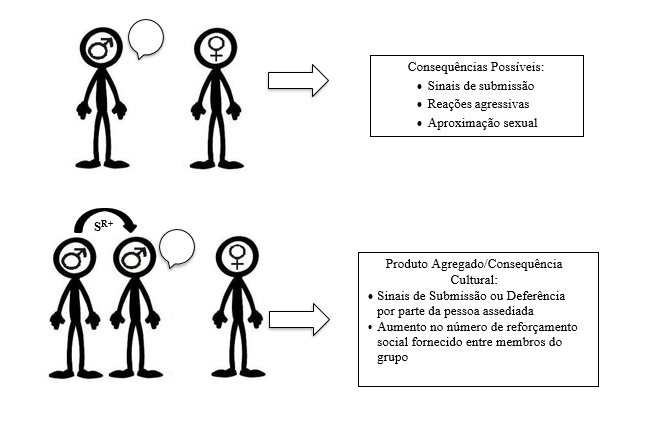
\includegraphics[width=1\textwidth]{7/figura2}
        \captionof{figure}{Esquema ilustrativo das possíveis contingências operantes e metacontingências envolvidas no assédio sexual verbal.}
        \label{figura2}
\end{center}
\end{figure}

Por outro lado, ao mesmo tempo que os comportamentos da vítima em relação aos comentários do assediador têm função de eventos selecionadores, a presença da vítima (estímulo discriminativo) em determinados locais, sob certas circunstâncias (estímulos condicionais, como estar sozinha ou em pequeno grupo), podem funcionar como eventos antecedentes para o comportamento de assédio. O Projeto \textit{Think Olga} (Hueck, 2017) e o \textit{Actionaid} (Câmara, 2016) fizeram dois levantamentos com 7.762 e 2.500 mulheres, respectivamente, questionando sobre assédios sofridos. O primeiro projeto aponta que 98\% das entrevistadas já sofreram com cantadas de rua no Brasil e o segundo sugere um índice de 86\% em quatro países (Brasil, Índia, Tailândia e Reino Unido). As situações de assédio podem ocorrer em locais públicos (ruas, praças, casa de show, praia, etc.) ou privados (residências, locais de trabalho, lojas, shoppings, escolas, etc.) e, geralmente, a vítima encontra-se sozinha ou em pequenos grupos.

Visto que os dois levantamentos citados indicam a ocorrência de assédio em diversos contextos, independente do ambiente físico ou do tipo de vestimenta da vítima, pode-se inferir que o comportamento do assediador seria evocado unicamente pela presença da mulher (estímulo antecedente para o assédio sexual verbal). Outros eventos ambientais passíveis de exercer controle discriminativo são estímulos que sinalizem a possibilidade de punição (e.g., a presença de um homem acompanhando a mulher; a presença de agentes de segurança pública; um grupo maior de mulheres, etc.), os quais inibiriam o assédio sexual verbal.

O levantamento do \textit{Think Olga} também possibilita algumas inferências sobre o comportamento das mulheres vítimas de assédio. Para 83\% das entrevistadas o assédio verbal é considerado desagradável (estímulo aversivo condicionado), mas apenas 27\% reage de alguma forma (contracontrole). Essas informações permitem supor que os sinais de submissão apresentados por grande parte das mulheres, assim como as reações agressivas, podem ser considerados comportamentos com função de fuga da estimulação verbal aversiva apresentada no episódio. Um dado que pode ajudar a explicar por que o contracontrole explícito só ocorre em cerca de 27\% dessas mulheres é o fato de que, dentre elas, 68\% relatam que foram agredidas verbalmente quando reagiram. Ou seja, mesmo tentando punir o comportamento do assediador, diversas vezes o assediador pune a reação da vítima. Um efeito a médio e longo prazo, também constatado no levantamento, é que 90\% das entrevistadas trocou de roupa e 81\% já deixou de fazer alguma coisa (ir a um lugar, passar na frente de uma obra, sair a pé) para evitar assédios. Ou seja, grande parte das vítimas entrevistadas desenvolveu repertórios de esquiva em relação às respostas verbais de assédio. A Figura \ref{figura3} ilustra possibilidades de análise funcional do comportamento da vítima e do assediador.

\begin{figure}[ht]
    \begin{center}
        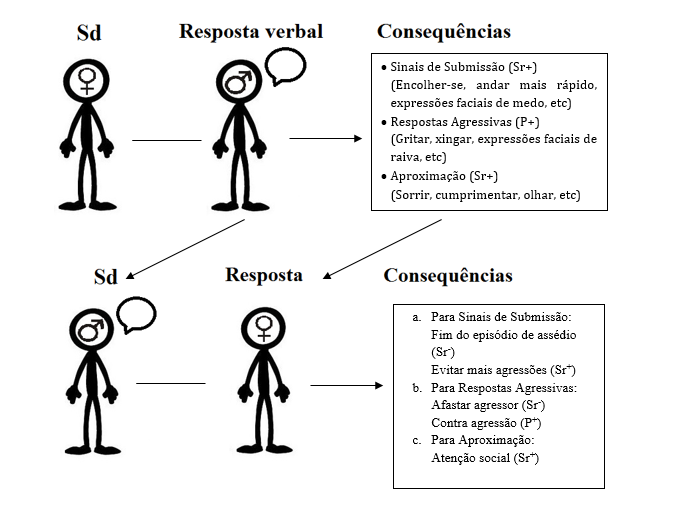
\includegraphics[width=1\textwidth]{7/figura3}
        \captionof{figure}{Análise molecular do comportamento operante de assédio do homem com suas possíveis consequências e comportamento operante que a vítima pode ter diante do assédio verbal e suas possíveis consequências.}
        \label{figura3}
\end{center}
\end{figure}

As mudanças nos repertórios comportamentais das mulheres (e.g., menos circulação em determinados locais, mudança no tipo de roupa usada, redução do engajamento em determinadas atividades para evitar assédio), que levam à restrição do acesso a diversos reforçadores, não afetam o comportamento dos assediadores, ou seja, não têm função seletiva (Glenn et al., 2016), dificultando a modificação da prática. Esta característica da prática do assédio a enquadra no conceito de macrocontingência, na qual cada operante individual e CCE tem suas consequências mantenedoras de forma independente dos efeitos cumulativos gerados (Figura \ref{figura4}).

\begin{figure}[ht]
    \begin{center}
        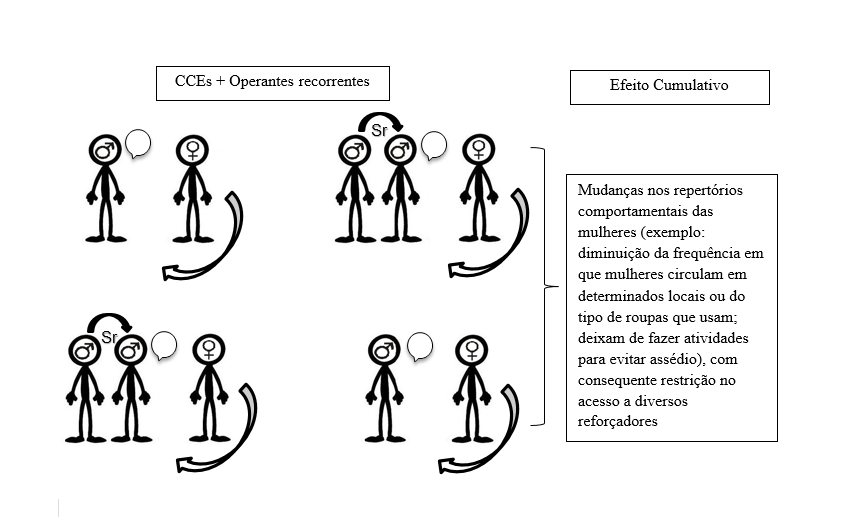
\includegraphics[width=1\textwidth]{7/figura4}
        \captionof{figure}{Esquema ilustrativo da macrocontingência que envolve a relação entre o macrocomportamento recorrente de assédio sexual verbal (representado pelo balão) e seu efeito cumulativo. As setas preenchidas indicam reforçamento social por pares. As setas vazadas indicam a recorrência do macrocomportamento.}
        \label{figura4}
\end{center}
\end{figure}

Considerando a falta de relação de contingência entre o macrocomportamento e o seu efeito cumulativo, conforme demonstrado nos exemplos anteriores, a literatura da área (Glenn, 2004; Glenn et al., 2016; Sampaio \& Andery, 2010) indica que intervenções devem ser planejadas de forma a estabelecer uma conexão entre o comportamento individual e seu efeito ou a impor custos para o comportamento local dos participantes da prática, por meio de contingências verbais que descrevam essa nova contingência (projetos de lei, fiscalizações, alteração do código penal, etc.). Espera-se que tais intervenções afetem a macrocontingência de forma que ocorra a redução na frequência da prática que a constitui, havendo também reduções no seu efeito cumulativo, a médio e longo prazo.

\section*{Modificando Práticas de Gênero}

Uma forma de controle do comportamento dentro de um Estado de direito é a promoção de regras sociais formais aprovadas pelo Poder Legislativo, as quais todos os cidadãos devem cumprir, sob pena de sofrerem sanções dos Poderes Executivo e/ou Judiciário. A aprovação de leis é um exemplo comum de intervenção sobre macrocomportamentos que visa estabelecer uma conexão – através de contingências verbais – entre o comportamento individual e/ou CCEs com seu efeito (Sampaio \& Andery, 2010; Glenn et al., 2016). De acordo com Skinner (1953/2005), contingências verbais desse tipo geralmente têm dois aspectos importantes: “Em primeiro lugar, especifica o comportamento. O comportamento em geral não é descrito topograficamente, mas em termos de seu efeito sobre outros – efeito que é objeto do controle governamental... Em segundo lugar, uma lei especifica ou dá a entender certa consequência, usualmente punição.” (Skinner, 1953/2005, p. 369).

No cenário legal brasileiro, está prevista no artigo nº 216 do Código Penal (Decreto-Lei nº. 2.848/1940) a punição para o assédio sexual que, segundo sua descrição, caracteriza-se por constrangimentos e ameaças feitas em local de trabalho por alguém em posição hierarquicamente superior à da vítima, com a finalidade de obter favores sexuais. A pena é de detenção e varia entre um e dois anos, caso o crime seja comprovado. A mesma legislação enquadra como ato obsceno (artigo 233) uma ação de cunho sexual (e.g., exibir seus genitais) em local público, a fim de constranger ou ameaçar alguém. A pena varia de três meses a um ano, ou pagamento de multa. Como pode ser visto, as formas de assédio sexual criminalizadas no país são bastante limitadas. No entanto, segundo alguns entendimentos legais, assédio pode ser considerado como qualquer conduta de natureza sexual indesejada pela vítima que, mesmo repelida por esta, é continuadamente reiterada, cerceando-lhe a liberdade sexual (Pamplona Filho, 2005).

Tendo em vista esse cenário, uma nova lei (projeto de Lei nº. 148 de 2017), mais ampla, sobre a questão do assédio foi aprovada em novembro de 2017 pela prefeitura do município de Fortaleza (Ceará). O texto prevê uma multa de R\$ 2.000,00 para a conduta de assédio em locais públicos ou privados, envolvendo comportamentos como ofender, intimidar, constranger ou hostilizar mulheres nas ruas e espaços privados da cidade, com palavras, gestos ou comportamentos, cabendo à Guarda Municipal registrar a ocorrência, assim como aplicar as sanções aos infratores. O valor arrecadado com a cobrança das multas será aplicado ao orçamento da Secretaria de Desenvolvimento Social, Direitos Humanos e Combate à Fome.

Vale destacar, contudo, que a existência da lei pode não ser suficiente para a alteração da macrocontingência de assédio, havendo a necessidade de adoção de estratégias para o cumprimento da mesma. Por exemplo, campanhas que deixem claro o que é um comportamento de assédio, evidenciando a contingência (e.g., enquanto uma repórter trabalha ao vivo, um torcedor desconhecido se aproxima e a beija rosto, após o quê ela demonstra insatisfação). Isso é importante para que a observação e análise do que é um comportamento de assédio seja compreendida partindo de um contexto, evitando a confusão com outros tipos de comportamentos de aproximação sexual considerados positivos (e.g., flerte, paquera, demonstração de afeto, etc.), deixando evidente qual desses comportamentos são puníveis pela lei.

Outra alternativa de modificação de práticas de gênero são iniciativas oriundas do movimento feminista. O movimento sufragista, iniciado na Grã-Bretanha e Estados Unidos no início do século XX, que lutou e conquistou o direito das mulheres ao voto, é um bom exemplo de alteração de macrocontingência. Esse processo teve uma longa duração e envolveu a criação de organizações compostas por mulheres (como o \textit{Women’s Social and Political Union}), além de publicações importantes como o livro \textit{A Vindication of the Rights of Woman}, de Mary Wollstonecraft (Abreu, 2002). No cenário brasileiro, após intensa campanha nacional, as mulheres adquiriram o direito de votar no ano de 1932 através do decreto nº 21.076, de 24 de fevereiro de 1932, e apenas no ano de 1990 o peso do eleitorado feminino foi igual ao masculino (Costa, 1991).

Um exemplo mais recente de modificação cultural está relacionado ao conceito de sororidade, que é considerada uma dimensão política, ética e prática do feminismo. Partindo da experiência individual feminina e sua busca por relações igualitárias, a sororidade é a construção de alianças de solidariedade entre mulheres e o desenvolvimento de uma consciência crítica sobre a cultura misógina existente, com o objetivo de diminuir as formas de opressão social (Gamba, 2007). Partindo desse conceito, foi criado o movimento “Vamos Juntas?” (Souza, 2016), iniciado pela jornalista Babi Souza, o qual foi impulsionado pela atual facilidade de contato com diversas pessoas por meio dos avanços tecnológicos. O movimento busca auxiliar as mulheres a se encontrarem, através de redes sociais, para que possam acompanhar umas às outras a determinados locais, diminuindo, assim, o risco de assédio sexual, visto que um número maior de mulheres pode reduzir a probabilidade de ocorrência desse tipo de situação, como analisado no presente trabalho.

\section*{Considerações Finais}

A Análise do Comportamento, principalmente a área de estudos sobre a cultura, seria beneficiada com mais estudos sobre as práticas de gênero, já estudadas por outras áreas de conhecimento (Couto \& Dittrich, 2017). Para isso, é fundamental analisar as variáveis envolvidas nos comportamentos, metacontingências e macrocontingências das práticas de gênero, assim como avaliar e promover formas efetivas de mudança social, visando um equilíbrio maior dos recursos da sociedade entre homens e mulheres (Malott \& Glenn, 2006; Ruiz, 2003). Skinner (1981), ao discutir a importância da Análise do Comportamento para lidar com problemas relacionados aos três níveis de seleção, ressalta que não reconhecer o papel da seleção por consequências implica em negligenciar as condições que precisam ser modificadas para resolver tais problemas. Além disso, apesar de não ser possível suprimir a seleção por consequências, pode-se arranjar contingências para modificar práticas culturais e, então, esperar que a seleção ocorra sobre estas práticas planejadas. As análises aqui apresentadas sobre práticas de gênero e sobre possíveis intervenções visam auxiliar o planejamento de futuros estudos e intervenções baseados na consideração da seleção no terceiro nível e em unidades de análise que têm se mostrado importantes ferramentas conceituais para o estudo da cultura.

Como já apontado por outras autoras (Couto \& Dittrich, 2017; Ruiz, 1995, 2003; Silva \& Laurenti, 2016), apesar dos muitos pontos em comum entre o Behaviorismo Radical e a literatura feminista, os estudos correlacionando as duas áreas são escassos. Destacamos que o cenário é ainda mais restrito quando se trata do uso de metacontingência e macrocontingência como unidades de análise. O presente trabalho visou, portanto, uma aproximação entre a literatura da Análise Comportamento da Cultura e os estudos sobre gênero, esperando-se que, com esta iniciativa, trabalhos futuros continuem a explorar as inter-relações existentes entre ambas, promovendo mudanças significativas, tanto acadêmicas, quanto sociais.

\section*{Referências Bibliográficas}\sectionmark{Referências Bibliográficas}

\hangindent=25pt
\hangafter=1
\noindent Abreu, Z. (2002). Luta das mulheres pelo direito ao voto: Movimentos sufragistas na Grã-Bretanha e Estados Unidos. \textit{Arquipelago História, 2}(6), 443-469. Recuperado de: \url{https://repositorio.uac.pt/handle/10400.3/380}

\hangindent=25pt
\hangafter=1
\noindent Alves, S. S. (2014). \textit{Saberes das mulheres veteranas na economia solidária: Sororidade a outra educação!} (Tese de Doutorado). Universidade Federal do Rio Grande do Sul, Porto Alegre, Rio Grande do Sul, Brasil.

\hangindent=25pt
\hangafter=1
\noindent Andery, M. A. P. A. (2010). Métodos de pesquisa em análise do comportamento. \textit{Psicologia USP, 21}(2), 313-342. Recuperado de \url{https://tinyurl.com/feminismo70}

\hangindent=25pt
\hangafter=1
\noindent Andrade, T. (2016). \textit{Mulheres no mercado de trabalho: Onde nasce a desigualdade?} Câmara dos Deputados. Consultoria Legislativa. Jul. 2016. Recuperado de \url{https://tinyurl.com/feminismo71}

\hangindent=25pt
\hangafter=1
\noindent Baum, W. M. (2006). \textit{Compreender o Behaviorismo: comportamento, cultura e evolução.} Ed 2. Artes Médicas: Porto Alegre, RS.

\hangindent=25pt
\hangafter=1
\noindent Câmara, J. (2016). \textit{Em pesquisa da ActionAid, 86\% das brasileiras ouvidas dizem já ter sofrido assédio em espaços urbanos.} Recuperado de: \url{https://tinyurl.com/feminismo72}

\hangindent=25pt
\hangafter=1
\noindent Costa, A. O. (1991). O acesso das mulheres à cidadania: questões em aberto. \textit{Caderno de Pesquisa, 77}, 47-52. Recuperado de: \url{https://tinyurl.com/feminismo73}

\hangindent=25pt
\hangafter=1
\noindent Couto, A. G., \& Dittrich, A. (2017). Feminismo e Análise do Comportamento: caminhos para o diálogo. \textit{Perspectivas em Análise do Comportamento, 8}(2), 147-158. Retirado de \url{https://tinyurl.com/feminismo74}

\hangindent=25pt
\hangafter=1
\noindent Daly, P. M. (1996). Sexism. In M. A. Mattaini \& B. A. Thyer (Eds.), \textit{Finding solutions to social problems: Behavioral strategies for change} (pp. 201-220). Washington, DC: American.

\hangindent=25pt
\hangafter=1
\noindent Decreto-lei nº 21.076, de 24 de Fevereiro de 1932. Decreta o Código Eleitoral. Diário Oficial da União, Brasília. 

\hangindent=25pt
\hangafter=1
\noindent Decreto-lei nº 2.848, de 07 de Dezembro de 1940. Regulamenta o Art. nº 216-A. Constranger alguém com o intuito de obter vantagem ou favorecimento sexual, prevalecendo-se o agente da sua condição de superior hierárquico ou ascendência inerentes ao exercício de emprego, cargo ou função (Incluído pela Lei nº 10.224, de 15 de 2001). Diário Oficial da União, Brasília.

\hangindent=25pt
\hangafter=1
\noindent Decreto-lei nº 3.688, de 03 de Outubro de 1941. Regulamenta o Art. 61. Importunar alguém, em lugar público ou acessível ao público, de modo ofensivo ao pudor. Diário Oficial da União, Brasília.

\hangindent=25pt
\hangafter=1
\noindent Fideles, M. N. D., \& Vandenberghe, L. (2014). Psicoterapia Analítica Funcional Feminista: possibilidades de um encontro. Psicologia: \textit{Teoria e Prática, 16}(3), 18-29. Recuperado de: \url{https://tinyurl.com/feminismo75}.

\hangindent=25pt
\hangafter=1
\noindent Gamba, S. B. (2007). \textit{Diccionario de Estudios de Género y Feminismos.} Buenos Aires: Ed. Biblos.

\hangindent=25pt
\hangafter=1
\noindent Glenn, S. S. (1986). Metacontingencies in Walden II. \textit{Behavior Analysis and Social Action, 5}, 2-8. Recuperado de \url{https://tinyurl.com/feminismo76}.

\hangindent=25pt
\hangafter=1
\noindent Glenn, S. S., Malott, M., Andery, M. A. P. A, Benvenuti, M., Houmanfar, R. A., Todorov, J. C., Tourinho, E. Z., Vasconcelos, L. A. (2016). Toward consistent terminology in a behaviorist approach to cultural analysis. \textit{Behavior and Social Issues, 25}, 11-27. Recuperado de \url{https://tinyurl.com/feminismo77}.

\hangindent=25pt
\hangafter=1
\noindent Hueck, K. (2017). \textit{Think Olga: Chega De Fiu Fiu.} Recuperado de: \url{https://tinyurl.com/feminismo78}

\hangindent=25pt
\hangafter=1
\noindent Instituto Brasileiro de Geografia e Estatística (2016). \textit{Pesquisa Nacional por Amostra de Domicílios: síntese de indicadores 2015}. Recuperado de \url{https://tinyurl.com/feminismo79}.

\hangindent=25pt
\hangafter=1
\noindent Malott, M. E., \& Glenn, S. S. (2006). Targets of intervention in cultural and behavioral change. \textit{Behavior and Social Issues, 15}(1), 31–56. doi: 10.5210/bsi.v15i1.344.

\hangindent=25pt
\hangafter=1
\noindent Muench, U., Sindelar, J., Busch, S. H., Peter, I., \& Buerhaus, P.I. (2015). Salary differences between male and female registered nurses in the United States. \textit{Journal of the American Medical Association, 313}(12), 1265-1267. doi:10.1001/jama.2015.1487 

\hangindent=25pt
\hangafter=1
\noindent Pamplona Filho, R. (2005). Assédio sexual: questões conceituais. \textit{Jus Navigandi, 704}(9). Recuperado de\\ \url{https://jus.com.br/artigos/6826/assedio-sexual}.

\hangindent=25pt
\hangafter=1
\noindent Pierce, W.D. (1991). Culture and society: the role of Behavioral Analysis. In: P.A. Lamal (Org.), \textit{Behavioral analysis of societies and cultural practices} (pp. 3-12). Nova Iorque: Hemisphere.

\hangindent=25pt
\hangafter=1
\noindent Ruiz, M. R. (1995). B. F. Skinner’s radical behaviorism: Historical misconstructions and grounds for feminist reconstructions. \textit{Behavior and Social Issues, 5}, 29-44.

\hangindent=25pt
\hangafter=1
\noindent Ruiz, M. R. (1998). Personal agency in feminist theory: Evicting the illusive dweller. \textit{The Behavior Analyst, 21}, 179–192.

\hangindent=25pt
\hangafter=1
\noindent Ruiz, M. R. (2003). Inconspicuous sources of behavioral control: the case of gendered practices. \textit{The Behavior Analyst Today, 4}, 12-16. Recuperado de\\ \url{http://psycnet.apa.org/record/2014-44018-002}.

\hangindent=25pt
\hangafter=1
\noindent Ruiz, M. R. (2009). Beyond the mirrored space: Time and resistance in feminist theory. \textit{Behavior and Philosophy, 37}, 141–147.

\hangindent=25pt
\hangafter=1
\noindent Ruiz, M. R., \& Roche, B. (2007). Values and the scientific culture of behavior analysis. \textit{The Behavior Analyst, 30}, 1–16.

\hangindent=25pt
\hangafter=1
\noindent Sá, C. P. (2016). J. G. Holland, contracontrole social e socialização do behaviorismo radical. \textit{Revista Brasileira de Terapia Comportamental e Cognitiva, 18}, 52-60.

\hangindent=25pt
\hangafter=1
\noindent Sadker, M. \& Sadker, D. (1994). \textit{Failing at fairness: How America’s schools cheat girls.} New York: Scribners.

\hangindent=25pt
\hangafter=1
\noindent Sampaio, A.A.S, \& Andery, M.A.P.A. (2010). Comportamento social, produção agregada e prática cultural: Uma análise comportamental de fenômenos sociais. \textit{Psicologia: Teoria e Pesquisa, 26}, 183-192. Recuperado de\\ \url{http://www.scielo.br/pdf/ptp/v26n1/a20v26n1.pdf}.

\hangindent=25pt
\hangafter=1
\noindent Sidman, M. (2009). \textit{Coerção e suas implicações} (M. A. P. A. Andery \& T. M. A. P. Sério, Trads.). Campinas, SP: Editora Livro Pleno. (Trabalho original publicado em 1989.).

\hangindent=25pt
\hangafter=1
\noindent Silva, F. B., \& Carrara, K. (2015). Implicações de estratégias molares/moleculares na Análise Comportamental da Cultura. \textit{Arquivos Brasileiros de Psicologia, 67}(3), 4-16. Recuperado de \url{https://tinyurl.com/feminismo70a}.

\hangindent=25pt
\hangafter=1
\noindent Silva, E. C., Laurenti, C. (2016). B. F. Skinner e Simone de Beauvoir: “a mulher” à luz do modelo de seleção por consequências. \textit{Perspectivas em Análise do Comportamento, 7}(2), 197-211. Recuperado de \url{https://www.revistaperspectivas.org/v7n2-a4}.

\hangindent=25pt
\hangafter=1
\noindent Skinner, B. F. (1981). Selection by consequences. \textit{Science, 213}, 501-504. Recuperado de \url{https://tinyurl.com/feminismo70b}

\hangindent=25pt
\hangafter=1
\noindent Skinner, B. F. (2005). \textit{Ciência e comportamento humano} (J. C. Todorov\& R. Azzi, Trads.). São Paulo: Martins Fontes. (Trabalho original publicado em 1953.)

\hangindent=25pt
\hangafter=1
\noindent Snustad, D. P., \& Simmons, M. J. (2012). \textit{Fundamentos da Genética.} Rio de Janeiro, RJ: Guanabara Koogan.

\hangindent=25pt
\hangafter=1
\noindent Souza, B. (2016). Vamos juntas? \textit{O guia de sororidade para todas.} Rio de Janeiro, RJ: Grupo Editorial Record. 

\hangindent=25pt
\hangafter=1
\noindent Studart, C. (2017). Projeto de Lei nº 0148 de 17 de abril de 2017. Estipula sanções para indivíduos que cometam assédio, assim como quaisquer atos que atentem contra a dignidade da Mulher no município de Fortaleza. Câmara Municipal de Fortaleza. Recuperado de: \url{https://tinyurl.com/feminismo70c}.

\hangindent=25pt
\hangafter=1
\noindent Todorov, J. C. (2012). Contingências de seleção cultural. \textit{Revista Brasileira de Análise do Comportamento, 8}(2), 95-105. Recuperado de \url{https://tinyurl.com/feminismo70d}.

\hangindent=25pt
\hangafter=1
\noindent Tourinho, E. Z. (2003). A produção de conhecimento em Psicologia: a Análise do Comportamento. \textit{Psicologia: Ciência e Profissão, 23}(2), 30-41. Recuperado de \url{www.tinyurl.com/feminismo70e}.

\hangindent=25pt
\hangafter=1
\noindent Wolpert, R. S. (2005). A multicultural feminist analysis of Walden II. \textit{The Behavior Analyst Today, 6}(3), 186-190. Recuperado de \url{http://psycnet.apa.org/fulltext/2014-44023-007.html}.